% Created 2014-01-23 jue 05:13
\documentclass[a4paper,12pt]{report}
\usepackage{fancyhdr}
\usepackage{lastpage}
\usepackage{extramarks}
\usepackage[usenames,dvipsnames]{color}
\usepackage{graphicx}
\usepackage{courier}
\usepackage{lipsum}
\usepackage{wrapfig}
\usepackage{geometry}
\usepackage{alltt}
\usepackage{textcomp}
\usepackage{ifthen}
\usepackage{adjustbox}
\usepackage[table]{xcolor}
\usepackage{caption}
\usepackage{subcaption}
\usepackage{hyperref}
\usepackage{titlesec}

\topmargin=-0.45in
\evensidemargin=0in
\oddsidemargin=0in
\textwidth=6.5in
\textheight=9.0in
\headsep=0.25in
\linespread{1.1}
\pagestyle{fancy}
\lhead{\hmwkLeft}
\chead{\hmwkCenter}
\rhead{\hmwkRight}
\lfoot{\lastxmark}
\cfoot{}
\rfoot{Página\ \thepage\ de\ \protect\pageref{LastPage}}
\renewcommand\headrulewidth{0.4pt}
\renewcommand\footrulewidth{0.4pt}
\setlength\parindent{0pt}
\setlength{\headheight}{15pt}
\definecolor{darkgreen}{rgb}{0.0,0.25,0.08}
\definecolor{ligthgreen}{rgb}{0.0,0.50,0.08}
\definecolor{Negro}{HTML}{000000}
\definecolor{listinggray}{gray}{0.9}
\definecolor{lbcolor}{rgb}{0.9,0.9,0.9}
\definecolor{darkblue}{rgb}{0,0.08,0.45}
\definecolor{malva}{HTML}{D28FFF}
\definecolor{azulito}{HTML}{62CDF5}
\hypersetup{
    colorlinks,
    citecolor=darkgreen,
    filecolor=darkgreen,
    linkcolor=darkgreen,
    urlcolor=darkgreen
}
\geometry{a4paper,tmargin=20mm,bmargin=20mm,lmargin=20mm,rmargin=20mm}
\titleformat{\chapter}[display]{\normalfont\huge\sffamily\bfseries\filcenter}{\vspace*{-2cm}
\leavevmode\leaders\vrule height7pt width3pt depth0pt
\hfill\kern8pt\thechapter\kern8pt
\leaders\vrule height7pt width3pt depth0pt\hfill}{3pt}{\vspace*{-5pt}\hrule\vspace{6pt}}[\vspace{1pt}\hrule\vspace{1cm}]
\newcommand\Bheadfont{\fontsize{11pt}{\baselineskip}\selectfont}
\titleformat{\section}[hang]{\normalfont\sc\color{darkblue}\Bheadfont}{\thesection\hskip0.618em}{0em}{}
\titlespacing*{\section}{0pt}{15pt plus 2pt minus 2pt}{9pt plus 2pt minus 2pt}
\titleformat{\subsection}[hang]{\normalfont\sc\color{darkgreen}}{\thesubsection\hskip0.618em}{0em}{}
\titlespacing*{\subsection}{0pt}{8pt plus 2pt minus 2pt}{8pt plus 2pt minus 2pt}
\titleformat{\subsubsection}[hang]{\normalfont\it}{}{0.618em}{}
\titlespacing*{\subsubsection}{0pt}{8pt plus 2pt minus 2pt}{4pt plus 2pt minus 2pt}
\title{
\vspace{2in}
\textmd{\textbf{\hmwkClass:\ \hmwkTitle}}\\
\normalsize\vspace{0.1in}\small{\hmwkDueDate}\\
\vspace{0.1in}\large{\textit{\hmwkClassInstructor\ }}
\vspace{3in}
}
\author{\textbf{\hmwkAuthorName}}
\date{}


\usepackage{fontspec}
\usepackage{minted}
\usepackage{pifont}
\usepackage{pstricks, pst-node}
\usemintedstyle{perldoc}
\usepackage[section]{placeins}
\renewcommand{\contentsname}{ÍNDICE}
\renewcommand{\chaptername}{C}
\newcommand{\hmwkLeft}{}
\newcommand{\hmwkCenter}{\hmwkClass}
\newcommand{\hmwkRight}{\hmwkTitle}
\newcommand{\hmwkTitle}{Proyecto DDSI}
\newcommand{\hmwkTitleExtended}{Sistema de Información para el registro y control de alimentos y dietas}
\newcommand{\hmwkClass}{Desarrollo De Sistemas de Información}
\newcommand{\hmwkClassInstructor}{}
\newcommand{\hmwkAuthorName}{}
\setmonofont[Scale=0.7]{Monaco}
\setmonofont[Scale=0.9]{FreeMono}
\usepackage{paralist}
\usepackage{slashbox}
\let\itemize\compactitem
\let\itemize\compactitem
\renewcommand{\bibname}{Referencias}
\renewcommand{\figurename}{Figura}
\renewcommand{\tablename}{Tabla}
\date{\today}
\title{Memoria}
\hypersetup{
  pdfkeywords={},
  pdfsubject={},
  pdfcreator={Emacs 24.3.1 (Org mode 8.2.4)}}
\begin{document}

\title{
\begin{center}
\vspace*{-2.5cm}
\begin{figure}[htb]
\begin{center}
\includegraphics[width=4cm]{/home/dabuti/University/ugr.jpg}
\end{center}
\end{figure}
\end{center}
\Huge{\textbf{Universidad de Granada}}\\
\vspace{1cm}
\Huge{\textbf{Grado en Ingeniería Informática}}\\
\vspace{2cm}
\hrule{}
\vspace{0.3cm}
\textbf{\hmwkClass}\\
\vspace{0.3cm}
\hrule{}
\vspace{2cm}
\textbf{\hmwkTitle}\\
\vspace{1cm}
\textbf{\hmwkTitleExtended}\\
\vspace{1.5cm}
\textbf{\small{Iris García de Sebastián}}\\
\textbf{\small{David Santiago Carrión}}\\
\vspace{0.1cm}
}

\maketitle
\clearpage
\tableofcontents
\clearpage

\chapter{Descripción}
\label{sec-1}
Se pretende implementar un sistema para registrar las comidas que se
llevan a cabo a lo largo del día y gestionar los alimentos. Para
ello se almacenarán los ingredientes que componen cada receta y su
cantidad, además de información nutricional acerca de cada alimento
y el lugar y precio donde lo adquirimos.


\section{Registro de alimentos}
\label{sec-1-1}
Al introducir los productos adquiridos en un supermercado estos
deben agruparse en categorías con un nivel de abstracción
superior, considerados como ingredientes. Por ejemplo si el
usuario compra una botella de aceite  de oliva 'Jucaso' en el
supermercado 'Coviran' y otra botella de aceite de oliva 'Borges'
en el supermercado Mercadona, ambos producto deben almacenarse en
el sistema bajo el producto 'aceite de oliva'.

De este modo cada producto que empleemos en la elaboración de
nuestra alimentación diaria está descrito por:
\begin{itemize}
\item \textbf{nombre del producto}: una serie de caracteres.
\item \textbf{energía}: un número que indica las kilocalorías que aporta por
cada 100 gramos de producto.
\item \textbf{Descripción}: detalles y explicaciones acerca del alimento.
\end{itemize}

Los alimentos los podemos adquirir en distintos establecimientos,
lo cual nos lleva a guardar información relevante acerca de los
mismos como:
\begin{itemize}
\item \textbf{nombre del establecimiento}: una serie de caracteres.
\item \textbf{dirección}: caracteres alfanuméricos que nos ayudan a ubicar la tienda.
\item \textbf{teléfono}: caracteres numéricos.
\item \textbf{web}: dirección web del comercio.
\end{itemize}

Tanto los datos de los alimentos como los de los supermercados
podrán ser modificados.


Cada vez que se hace una compra se registra información de los
productos adquiridos:
\begin{itemize}
\item \textbf{producto}: el producto comprado.
\item \textbf{establecimiento}: donde lo hemos comprado.
\item \textbf{comprador}: el usuario que ha realizado la compra.
\item \textbf{cantidad}: número de unidades adquiridas del producto.
\item \textbf{precio}: número que indica el coste total.
\item \textbf{fecha}: cuando se realizó la adquisición.
\end{itemize}

\section{Registro de dietas}
\label{sec-1-2}
Con todos los ingredientes adquirdos se pueden cocinar recetas. Las
recetas se describen y se almacena en el sistema teniendo en cuenta
los siguientes puntos:
\begin{itemize}
\item \textbf{nombre}: una serie de caracteres.
\item \textbf{personas}: número de comensales a los que puede abastecer.
\item \textbf{ingredientes}: un conjunto formado por los alimentos necesarios.
\item \textbf{cantidad}: indica la proporción de cada ingrediente.
\item \textbf{tiempo}: minutos que nos puede costar cocinarlo.
\item \textbf{valor nutricional}: número total de calorías que aporta la
receta.
\item \textbf{descripción}: documento que indica los pasos a seguir para
realizar el plato.
\end{itemize}

\vspace{0.2cm}
A partir de las diferentes recetas se pueden crear listas
personalizadas de las mismas, generando dietas. Las dietas son
creadas por los usuarios y les pertenecen a ellos exclusivamente. A
diferencia de las recetas estas no se comparten.

Se guardarán los siguientes puntos:
\begin{itemize}
\item \textbf{nombre de la dieta}: una serie de caracteres.
\item \textbf{recetas}: el conjunto de recetas asociado a la dieta.
\item \textbf{descripción}: información adicional sobre la dieta descrita.
\item \textbf{usuario}: identifica al propietario de la dieta.
\end{itemize}

\vspace{0.2cm}
Tanto las recetas como las dietas han de poder ser editadas,
eliminando y agregando ingredientes o recetas según el caso.

Dada una dieta en concreto, se listará la información general de la
misma junto con sus recetas asociadas, permitiendo al usuario
hacerse una idea de los platos que puede preparar.

Cada vez que alguien realiza una receta se registra quien cocinó la
comida, para llevar un control de la despensa:
\begin{itemize}
\item \textbf{Usuario}: quien la ha cocinado.
\item \textbf{Receta}: que receta se ha cocinado.
\item \textbf{Fecha}: cuando se ha realizado la comida.
\end{itemize}

\vspace{0.2cm}
Los usuarios podrán ver los platos que han realizado y se les
ofrecerá la opción de eliminar una comida registrada, para subsanar
posibles errores de registro.

\section{Registro de usuarios}
\label{sec-1-3}
La base de usuarios estarán registrados, permitiendoles realizar
dietas específicas, comidas, compras o recetas. Sus datos serían:
\begin{itemize}
\item \textbf{nombre}: una serie de caracteres.
\item \textbf{primer apellido}: caracteres alfabéticos.
\item \textbf{segundo apellido}:  una serie de caracteres.
\item \textbf{nick}: caracteres por los que quiere ser identificado.
\item \textbf{contraseña}: combinación necesaria para entrar al sistema.
\end{itemize}

\vspace{0.2cm}
Los usuarios anónimos tienen la opción de darse de alta en el
sistema proporcionando los datos previamente expuestos. A partir de
entonces podrán acceder a las distintas operaciones que ofrece el
sistema, así como editar o eliminar su perfil.


\section{Información y estadísticas}
\label{sec-1-4}
Los usuarios del sistema tienen acceso a información extraida de
las acciones que han ido llevando a cabo con el uso cotidiano del
sistema.

De este modo podrán acceder a una lista con todos los alimentos que
tienen disponibles actualmente en la despensa y a una lista de
recetas que pueden ser cocinadas en vista de los ingredientes con
los que cuenta y las dietas que ha creado.

Cuando un usuario crea una dieta y asocia los platos que desea,
podrá obtener el coste que le supondría adquirir los productos, en
los distintos supermercados, para ejecutar todos los platos de
dicha dieta.

Por último, el usuario deberá poder obtener su gasto medio en
euros, tanto diario como mensual.
\chapter{Análisis de requisitos}
\label{sec-2}
\section{Requisitos de datos}
\label{sec-2-1}
\subsection{RD-1: Datos nuevo producto}
\label{sec-2-1-1}
\begin{itemize}
\item \textbf{Nombre}: una cadena de hasta 20 caracteres no vacía.
\item \textbf{Calorías}: un número decimal positivo.
\item \textbf{Descripción}: una cadena de hasta 200 caracteres.
\end{itemize}

\subsection{RD2-Datos producto:}
\label{sec-2-1-2}
\begin{itemize}
\item \textbf{Identificador} de producto: un número entero.
\item \textbf{Nombre}: una cadena de hasta 20 caracteres no vacía.
\item \textbf{Calorías}: un número decimal positivo.
\item \textbf{Descripción}: una cadena de hasta 200 caracteres.
\end{itemize}
\subsection{RD3-Datos producto modificado:}
\label{sec-2-1-3}
\begin{itemize}
\item \textbf{Identificador} de producto: un número entero.
\item \textbf{Nombre}: una cadena de hasta 20 caracteres.
\item \textbf{Calorías}: un número decimal positivo.
\item \textbf{Descripción}: una cadena de hasta 200 caracteres.
\end{itemize}
\subsection{RD4-Identificador comprador:}
\label{sec-2-1-4}
\begin{itemize}
\item \textbf{Identificador} de usuario: un número entero.
\end{itemize}
\subsection{RD5-Lista de productos comprados:}
\label{sec-2-1-5}
\begin{itemize}
\item \textbf{Identificador} de producto: un número entero.
\item \textbf{Nombre}: una cadena de hasta 20 caracteres no vacía.
\item \textbf{Calorías}: un número decimal positivo.
\item \textbf{Descripción}: una cadena de hasta 200 caracteres.
\end{itemize}
\subsection{RD6-Datos nuevo super:}
\label{sec-2-1-6}
\begin{itemize}
\item \textbf{Nombre}:  una cadena de hasta 20 caracteres no vacía.
\item \textbf{Dirección}:  una cadena de hasta 30 caracteres no vacía.
\item \textbf{Teléfono}: una cadena de 9 caracteres numéricos.
\item \textbf{Página} web: una cadena de hasta 20 caracteres no vacía.
\end{itemize}
\subsection{RD7-Datos super:}
\label{sec-2-1-7}
\begin{itemize}
\item \textbf{Identificador} de super: un número entero.
\item \textbf{Nombre}:  una cadena de hasta 20 caracteres no vacía.
\item \textbf{Dirección}:  una cadena de hasta 30 caracteres.
\item \textbf{Teléfono}: una cadena de hasta 9 caracteres numéricos.
\item \textbf{Página web}: una cadena de hasta 20 caracteres.
\end{itemize}
\subsection{RD8-Datos super modificado:}
\label{sec-2-1-8}
\begin{itemize}
\item \textbf{Identificador de super}: un número entero.
\item \textbf{Nombre}:  una cadena de hasta 20 caracteres.
\item \textbf{Dirección}:  una cadena de hasta 30 caracteres.
\item \textbf{Teléfono}: una cadena de hasta 9 caracteres numéricos.
\item \textbf{Página web}: una cadena de hasta 20 caracteres.
\end{itemize}
\subsection{RD9-Datos nueva compra:}
\label{sec-2-1-9}
\begin{itemize}
\item \textbf{Identificador} de usuario: un número entero.
\end{itemize}

\subsection{RD10-Datos compra:}
\label{sec-2-1-10}
\begin{itemize}
\item \textbf{Identificador de compra}: un número entero.
\item \textbf{Identificador de usuario}: un número entero.
\item \textbf{Fecha}: tres conjuntos de enteros formados los dos primeros por conjuntos de dos cifras y el                 tercero por un conjunto de cuatro cifras, separados por barras ('/').
\end{itemize}
\subsection{RD11-Datos nueva línea de compra:}
\label{sec-2-1-11}
\begin{itemize}
\item \textbf{Identificador de compra}: un número entero.
\item \textbf{Identificador de producto}: un número entero.
\item \textbf{Identificador de super}: un número entero.
\item \textbf{Cantidad}: un número entero mayor que cero.
\item \textbf{Importe}: un número decimal mayor que cero.
\end{itemize}
\subsection{RD12-Datos línea de compra:}
\label{sec-2-1-12}
\begin{itemize}
\item \textbf{Identificador de compra}: un número entero.
\item \textbf{Identificador de producto}: un número entero.
\item \textbf{Identificador de super}: un número entero.
\item \textbf{Cantidad}: un número entero mayor que cero.
\item \textbf{Importe}: un número decimal mayor que cero.
\end{itemize}
\subsection{RD13-Datos línea de compra a eliminar:}
\label{sec-2-1-13}
\begin{itemize}
\item \textbf{Identificador de compra}: un número entero.
\item \textbf{Identificador de producto}: un número entero.
\item \textbf{Identificador de super}: un número entero.
\end{itemize}
\subsection{RD14-Datos nueva dieta:}
\label{sec-2-1-14}
\begin{itemize}
\item \textbf{Identificador de usuario}: un número entero.
\item \textbf{Nombre}: una cadena de hasta 20 caracteres no vacía.
\item \textbf{Descripción}: una cadena de hasta 200 caracteres.
\end{itemize}
\subsection{RD15-Datos dieta:}
\label{sec-2-1-15}
\begin{itemize}
\item \textbf{Identificador de dieta}: un número entero.
\item \textbf{Identificador de usuario}: un número entero.
\item \textbf{Nombre}: una cadena de hasta 20 caracteres no vacía.
\item \textbf{Descripción}: una cadena de hasta 200 caracteres.
\end{itemize}
\subsection{RD16-Datos nueva receta de dieta:}
\label{sec-2-1-16}
\begin{itemize}
\item \textbf{Identificador de dieta}: un número entero.
\item \textbf{Identificador de receta}: un número entero.
\end{itemize}
\subsection{RD17-Datos receta de dieta:}
\label{sec-2-1-17}
\begin{itemize}
\item \textbf{Identificador de dieta}: un número entero.
\item \textbf{Identificador de receta}: un número entero.
\end{itemize}
\subsection{RD18-Datos receta de dieta a eliminar:}
\label{sec-2-1-18}
\begin{itemize}
\item \textbf{Identificador de dieta}: un número entero.
\item \textbf{Identificador de receta}: un número entero.
\end{itemize}
\subsection{RD19-Datos nueva receta:}
\label{sec-2-1-19}
\begin{itemize}
\item \textbf{Nombre}: una cadena de hasta 20 caracteres no vacía.
\item \textbf{Personas}: un número entero.
\item \textbf{Tiempo}: un número entero.
\item \textbf{Descripción}: una cadena de hasta 200 caracteres.
\end{itemize}
\subsection{RD20-Datos receta:}
\label{sec-2-1-20}
\begin{itemize}
\item \textbf{Identificador de receta}: un número entero.
\item \textbf{Nombre}: una cadena de hasta 20 caracteres no vacía.
\item \textbf{Personas}: un número entero mayor que cero.
\item \textbf{Tiempo}: un número entero mayor que cero.
\item \textbf{Descripción}: una cadena de hasta 200 caracteres.
\end{itemize}
\subsection{RD21-Datos nuevo producto de receta:}
\label{sec-2-1-21}
\begin{itemize}
\item \textbf{Identificador de producto}: un número entero.
\item \textbf{Identificador de receta}: un número entero.
\item \textbf{Cantidad}: un número entero.
\end{itemize}
\subsection{RD22-Datos producto de receta:}
\label{sec-2-1-22}
\begin{itemize}
\item \textbf{Identificador de producto}: un número entero.
\item \textbf{Identificador de receta}: un número entero.
\item \textbf{Cantidad}: un número entero.
\end{itemize}
\subsection{RD23-Datos producto de receta a eliminar:}
\label{sec-2-1-23}
\begin{itemize}
\item Identificador de producto: un número entero.
\item Identificador de receta: un número entero.
\end{itemize}
\subsection{RD24-Datos receta modificada:}
\label{sec-2-1-24}
\begin{itemize}
\item Identificador de receta: un número entero.
\item Nombre: una cadena de hasta 20 caracteres.
\item Personas: un número entero.
\item Tiempo: un número entero.
\item Descripción: una cadena de hasta 200 caracteres.
\end{itemize}
\subsection{RD25-Datos nuevo usuario:}
\label{sec-2-1-25}
\begin{itemize}
\item Nombre: una cadena de hasta 20 caracteres no vacía.
\item Primer apellido: una cadena de hasta 20 caracteres.
\item Segundo apellido: una cadena de hasta 20 caracteres.
\item Nombre de usuario: una cadena de hasta 20 caracteres.
\item Contraseña: una cadena alfanumérica de hasta 20 elementos.
\end{itemize}
\subsection{RD26-Datos usuario:}
\label{sec-2-1-26}
\begin{itemize}
\item Identificador de usuario: un número entero.
\item Nombre: una cadena de hasta 20 caracteres no vacía.
\item Primer apellido: una cadena de hasta 20 caracteres.
\item Segundo apellido: una cadena de hasta 20 caracteres.
\item Nombre de usuario: una cadena de hasta 20 caracteres.
\item Contraseña: una cadena alfanumérica de hasta 20 elementos.
\end{itemize}
\subsection{RD27-Datos usuario modificado:}
\label{sec-2-1-27}
\begin{itemize}
\item Identificador de usuario: un número entero.
\item Nombre: una cadena de hasta 20 caracteres no vacía.
\item Primer apellido: una cadena de hasta 20 caracteres.
\item Segundo apellido: una cadena de hasta 20 caracteres.
\item Contraseña: una cadena alfanumérica de hasta 20 elementos.
\end{itemize}

\subsection{RD28-Datos usuario a eliminar:}
\label{sec-2-1-28}
\begin{itemize}
\item Identificador de usuario: un número entero.
\end{itemize}
\subsection{RD29-Datos nueva comida:}
\label{sec-2-1-29}
\begin{itemize}
\item Identificador de usuario: un número entero.
\item Identificador de receta: un número entero.
\item Fecha: tres conjuntos de enteros formados los dos primeros por conjuntos de dos cifras y el                 tercero por un conjunto de cuatro cifras, separados por barras ('/').
\end{itemize}
\subsection{RD30-Datos comida:}
\label{sec-2-1-30}
\begin{itemize}
\item Identificador de usuario: un número entero.
\item Identificador de receta: un número entero.
\item Fecha: tres conjuntos de enteros formados los dos primeros por conjuntos de dos cifras y el                 tercero por un conjunto de cuatro cifras, separados por barras ('/').
\end{itemize}
\subsection{RD31-Identificador propietario de stock:}
\label{sec-2-1-31}
\begin{itemize}
\item Identificador de usuario: un número entero.
\end{itemize}
\subsection{RD32-Lista de stock:}
\label{sec-2-1-32}
\begin{itemize}
\item Identificador de producto: un número entero.
\item Nombre: una cadena de hasta 20 caracteres no vacía.
\item Calorías: un número decimal positivo.
\item Descripción: una cadena de hasta 200 caracteres.
\item Cantidad: un número entero mayor que cero.
\end{itemize}
\subsection{RD33-Identificador usuario para gasto diario:}
\label{sec-2-1-33}
\begin{itemize}
\item Identificador de usuario: un número entero.
\end{itemize}
\subsection{RD34-Valor de gasto diario:}
\label{sec-2-1-34}
\begin{itemize}
\item Gasto: un número decimal.
\end{itemize}
\subsection{RD35-Identificador usuario para gasto mensual:}
\label{sec-2-1-35}
\begin{itemize}
\item Identificador de usuario: un número entero.
\end{itemize}
\subsection{RD36-Valor de gasto mensual:}
\label{sec-2-1-36}
\begin{itemize}
\item Gasto: un número decimal.
\end{itemize}
\subsection{RD37-Usuario que consulta recetas disponibles:}
\label{sec-2-1-37}
\begin{itemize}
\item Identificador de usuario: un número entero.
\end{itemize}
\subsection{RD38-Lista recetas disponibles:}
\label{sec-2-1-38}
\begin{itemize}
\item Identificador de receta: un número entero.
\item Nombre: una cadena de hasta 20 caracteres no vacía.
\item Personas: un número entero mayor que cero.
\item Tiempo: un número entero mayor que cero.
\item Descripción: una cadena de hasta 200 caracteres.
\end{itemize}
\subsection{RD39-Identificador de dieta a consultar:}
\label{sec-2-1-39}
\begin{itemize}
\item Identificador de dieta: un número entero.
\end{itemize}
\subsection{RD40-Coste por super:}
\label{sec-2-1-40}
\begin{itemize}
\item Identificador de super: un número entero.
\item Nombre:  una cadena de hasta 20 caracteres no vacía.
\item Dirección:  una cadena de hasta 30 caracteres.
\item Teléfono: una cadena de hasta 9 caracteres numéricos.
\item Página web: una cadena de hasta 20 caracteres.
\item Gasto: un número decimal.
\end{itemize}
\subsection{RD41-Datos de identificación:}
\label{sec-2-1-41}
\begin{itemize}
\item Nombre: una cadena de hasta 20 caracteres no vacía.
\item Contraseña: una cadena alfanumérica de hasta 20 elementos no vacía.
\end{itemize}
\subsection{RD42-Identificador creador de dieta completa:}
\label{sec-2-1-42}
\begin{itemize}
\item Identificador de usuario: un número entero.
\end{itemize}
\subsection{RD43-Datos dieta completa:}
\label{sec-2-1-43}
\begin{itemize}
\item Identificador de dieta: un número entero.
\item Nombre: una cadena de hasta 20 caracteres no vacía.
\item Descripción: una cadena de hasta 200 caracteres.
\end{itemize}
\subsection{RD44-Lista de recetas de dieta:}
\label{sec-2-1-44}
\begin{itemize}
\item Identificador de receta: un número entero.
\item Nombre: una cadena de hasta 20 caracteres.
\item Personas: un número entero.
\item Tiempo: un número entero.
\item Descripción: una cadena de hasta 200 caracteres.
\end{itemize}
\subsection{RD45-Identificador creador de dietas:}
\label{sec-2-1-45}
\begin{itemize}
\item Identificador de usuario: un número entero.
\end{itemize}
\subsection{RD46-Lista de dietas:}
\label{sec-2-1-46}
\begin{itemize}
\item Identificador de dieta: un número entero.
\item Nombre: una cadena de hasta 20 caracteres no vacía.
\item Descripción: una cadena de hasta 200 caracteres.
\end{itemize}
\subsection{RD47-Identificador consultor de recetas:}
\label{sec-2-1-47}
\begin{itemize}
\item Identificador de usuario: un número entero.
\end{itemize}
\subsection{RD48-Lista de recetas:}
\label{sec-2-1-48}
\begin{itemize}
\item Identificador de receta: un número entero.
\item Nombre: una cadena de hasta 20 caracteres.
\item Personas: un número entero.
\item Tiempo: un número entero.
\item Descripción: una cadena de hasta 200 caracteres.
\end{itemize}
\subsection{RD49-Identificador usuario propio:}
\label{sec-2-1-49}
\begin{itemize}
\item Identificador de usuario: un número entero.
\end{itemize}
\subsection{RD50-Datos usuario propio:}
\label{sec-2-1-50}
\begin{itemize}
\item Nombre: una cadena de hasta 20 caracteres.
\item Primer apellido: una cadena de hasta 20 caracteres.
\item Segundo apellido: una cadena de hasta 20 caracteres.
\item Nombre de usuario: una cadena de hasta 20 caracteres.
\item Contraseña: una cadena alfanumérica de hasta 20 elementos.
\end{itemize}
\subsection{RD51-Identificador cocinero:}
\label{sec-2-1-51}
\begin{itemize}
\item Identificador de usuario: un número entero.
\end{itemize}
\subsection{RD52-Lista de comidas:}
\label{sec-2-1-52}
\begin{itemize}
\item Identificador de usuario: un número entero.
\item Identificador de receta: un número entero.
\item Fecha: tres conjuntos de enteros formados los dos primeros por
conjuntos de dos cifras y el tercero por un conjunto de cuatro
cifras, separados por barras ('/').
\end{itemize}
\subsection{RD53-Datos comida a eliminar:}
\label{sec-2-1-53}
\begin{itemize}
\item Identificador de usuario: un número entero.
\item Identificador de receta: un número entero.
\item Fecha: tres conjuntos de enteros formados los dos primeros por
conjuntos de dos cifras y el tercero por un conjunto de cuatro
cifras, separados por barras ('/').
\end{itemize}

\section{Requisitos funcionales}
\label{sec-2-2}
\section{Restricciones semánticas}
\label{sec-2-3}
\chapter{Esquema caja negra}
\label{sec-3}
\chapter{Refinamiento 0}
\label{sec-4}
\section{DFD 0 (Esquema Armazón)}
\label{sec-4-1}
\section{Esquema externo 0}
\label{sec-4-2}
\section{Entidad Relación 0}
\label{sec-4-3}
\chapter{Refinamiento 1}
\label{sec-5}
\section{DFD 1}
\label{sec-5-1}
\section{Esquema externo 1}
\label{sec-5-2}
\section{Entidad Relación 1}
\label{sec-5-3}
\chapter{Refinamiento 2}
\label{sec-6}
\section{DFD 2 (Esquema Armazón)}
\label{sec-6-1}
\section{Esquema externo 2}
\label{sec-6-2}
\section{Entidad Relación 2}
\label{sec-6-3}
\section{Entidad Relación final (atributos)}
\label{sec-6-4}
\chapter{Esquemas de Operación y Navegación}
\label{sec-7}
\section{Proceso: Gestión Usuarios}
\label{sec-7-1}
\subsection{Lista de operaciones:}
\label{sec-7-1-1}
\begin{enumerate}
\item Listar los productos comprados por un usuario
\begin{itemize}
\item Esquema de operación:
\begin{figure}[!htp]
\centering
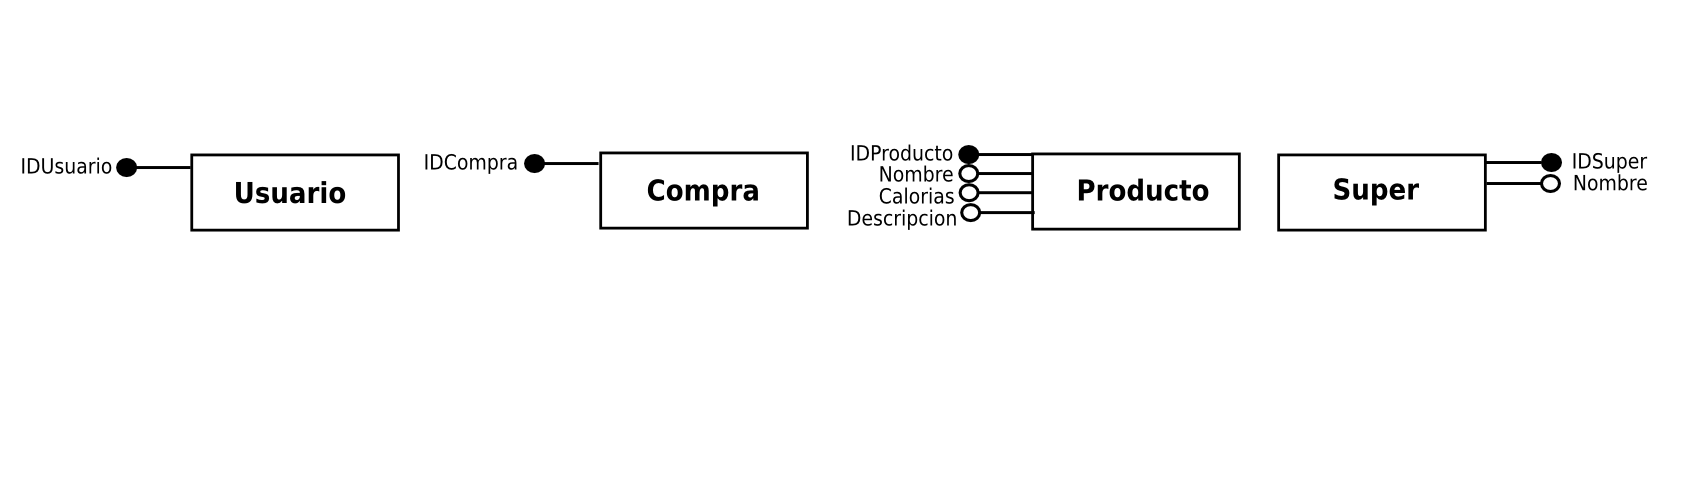
\includegraphics[width=0.9\linewidth]{./operaciones/img/ope01.png}
\caption{Esquema Operación - 01}
\label{fig:ope01}
\medskip
\footnotesize
{}
\end{figure}
\item Esquema de navegación:
\begin{figure}[!htp]
\centering
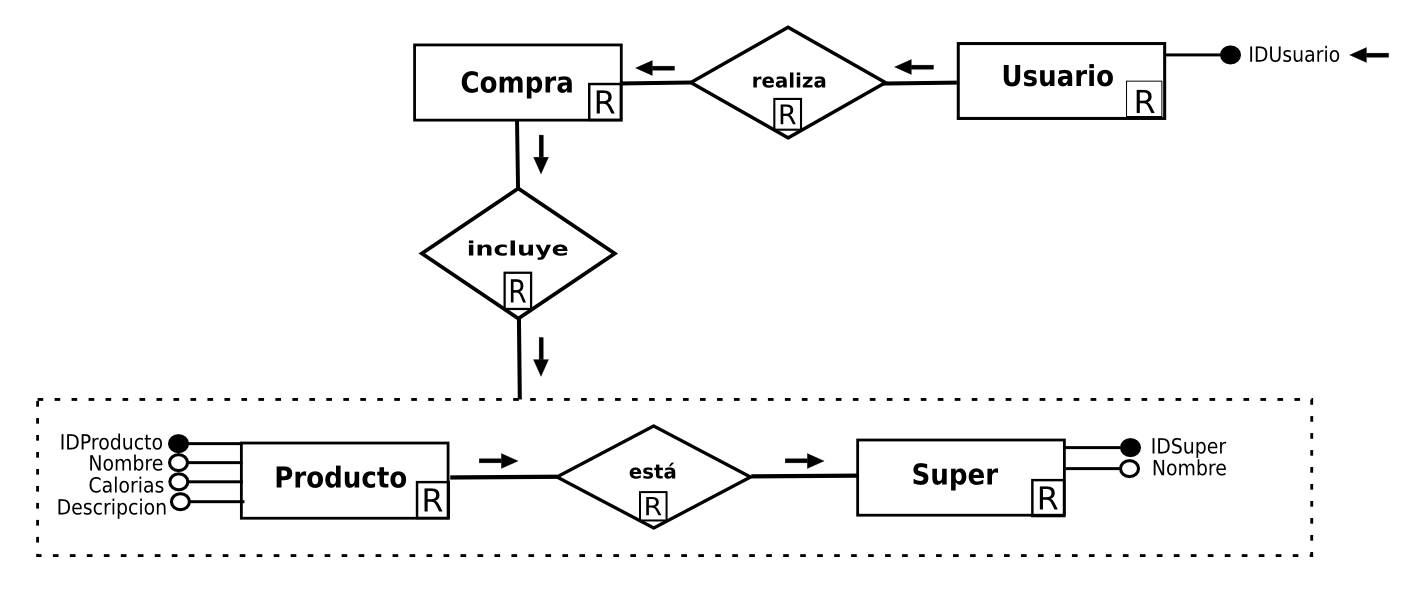
\includegraphics[width=0.9\linewidth]{./operaciones/img/nave01.png}
\caption{Esquema Operación - 01}
\label{fig:ope01}
\medskip
\footnotesize
{}
\end{figure}
\end{itemize}
\item Modificar un nuevo usuario a partir de su nombre, apellido1,
apellido2, username y password.
\end{enumerate}

\section{Proceso: \ldots{}}
\label{sec-7-2}
\subsection{Lista de operaciones:}
\label{sec-7-2-1}
Descripción\ldots{}
\begin{itemize}
\item Esquema operación:
includegraphics
\item Esquema navegación:
includegraphics
\end{itemize}
\chapter{Interface}
\label{sec-8}

\chapter{Manual de usuario}
\label{sec-9}
% Emacs 24.3.1 (Org mode 8.2.4)
\end{document}
